\documentclass[a4paper]{article}
%\usepackage{fourier-otf}
\usepackage[utf8]{inputenc}
\usepackage{graphicx}
\usepackage{algorithm}
\usepackage{algpseudocode}
\usepackage{multirow}
\usepackage{float}
\usepackage{lipsum}
\usepackage{scrextend}
\usepackage{biblatex}
\addbibresource{bibliography.bib}
\usepackage{listings}
\usepackage{amsmath}
\usepackage{amsfonts}
%\usepackage[square,sort,comma,numbers]{natbib}
\newtheorem{theorem}{Theorem}[section]
\usepackage{color}
\usepackage{makeidx}
\usepackage{titlepic}
\newtheorem{remark}{Remark}
\definecolor{mygreen}{rgb}{0,0.6,0}
\definecolor{mygray}{rgb}{0.5,0.5,0.5}
\definecolor{mymauve}{rgb}{0.58,0,0.82}
\lstset{ %
	backgroundcolor=\color{white},   % choose the background color
	basicstyle=\footnotesize,        % size of fonts used for the code
	breaklines=true,                 % automatic line breaking only at whitespace
	captionpos=b,                    % sets the caption-position to bottom
	commentstyle=\color{mygreen},    % comment style
	escapeinside={\%*}{*)},          % if you want to add LaTeX within your code
	keywordstyle=\color{blue},       % keyword style
	stringstyle=\color{mymauve},     % string literal style
}
\usepackage{hyperref}
\hypersetup{
  colorlinks   = true,    % Colours links instead of ugly boxes
  urlcolor     = black,    % Colour for external hyperlinks
  linkcolor    = black,    % Colour of internal links
  citecolor    = black      % Colour of citations
}
%\title{First chapter}

%\author{F.Bernardi}

%\protect\\ 

\newcommand{\myName}{Fabrizio Bernardi}
\newcommand{\myTitle}{Modeling and data analysis of the calcium activity in somatostatin interneurons from in vivo imaging on mice }
\newcommand{\myDegree}{Programme: \protect\\ \textit{Mathematical Engineering}}
\newcommand{\myCycle}{XXXI cycle}
\newcommand{\myDepartment}{Department of Mathematics}
\newcommand{\myUni}{Politecnico di Milano}
\newcommand{\myYear}{2022}
\newcommand{\myTime}{01 Jan \myYear}

\pdfbookmark{Cover}{cover}

\begin{document}
	

	
\section{Mathematical modeling in cellular electrophysiology}

In Section 1.1, the concept of \textit{excitability} of neurons has been introduced: neurons are able to generate and transmit \textbf{electrical impulses} as a response to external stimuli. These impulses are a direct consequence of rapid changes in intracellular end extracellular \textit{ionic concentrations} of main chemicals such as $Na^+, Cl^-, K^+, Ca^{2+}$. The change of such concentration values determines a change in the electric potential difference formed across the cell's membrane, and thus the formation of an \textbf{action potential}. \\
In this chapter, mathematical models to describe cellular electric activity are presented. After introducing the main assumptions of the models, the equivalent circuit formulations for cellular electrophyioslogy will be presented, along with different ways to describe its electrical components. Finally, the main model to describe the propagation of the action potential between two neurons will be considered, namely the \textbf{cable equation model}. All these models consist in either \textbf{ordinary differential equations (ODEs)} or \textbf{partial differential equations (PDEs)}, to be numerically solved through appropriate techniques, briefly discussed in the final part of the chapter.

\subsection{Electric activity in neurons}


\begin{figure}[H]
	\begin{center}
		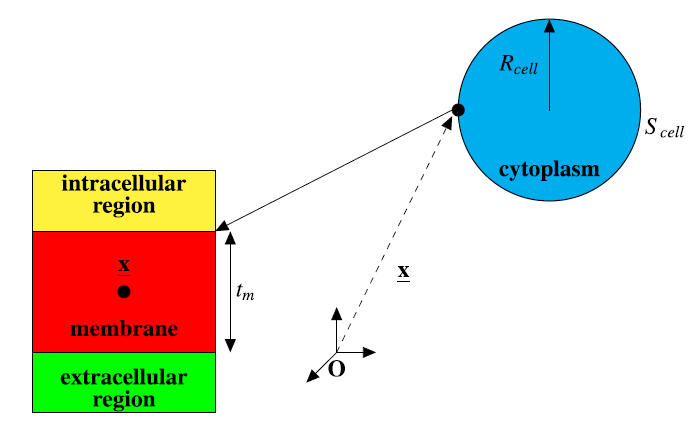
\includegraphics[scale=0.77]{first.png} 
	\end{center} 
	\caption{\textit{Schematic model of a cell with a focus on a local point $\textbf{x}$ of the membrane}}
	
\end{figure}




In order to mathematically describe the main electric functionalities of a cell, we first need to understand the set of phenomena which characterize this complex component of our body, such as the processes leading to its condition of \textit{dynamical equilibirium}, called the \textbf{cellular homeostasis}. The cellular homeostasis is achieved through the equilibrium of several forces acting on the cell, which can be of fluid, mechanical, chemical or electric nature, although the focus in this work will regard only the elctrical part.\\
The \textit{intracellular} environment of a cell consists mainly in a water solution contaning vital nutrients and elements in ionic form such as  $Na^+, Cl^-, K^+, Ca^{2+}$, making the solution behaving like a charged fluid. The intracellular environment is separated by the extracellular one by the \textbf{membrane} of the cell (see Figure). The membrane is formed by a bilayer of lipids (of thickness considerably smaller than the cell's radius) which does not allow passage of substances through it. The passage of some ions is still allowed through specific sites called \textbf{ionic channels}, each of one allowing, under certain conditions, the passage of a single ionic species. The movement of one ionic species from the intracellular to the extracellular environment, or viceversa, is caused by the different concentration of such quantity in the two regions, leading to an \textit{electrochemical gradient} which forces positive charges to move from high to low potentials, and thus forming a potential difference across the membrane. We call this quantity the \textbf{membrane potential} of the cell. The main role of the mathematical models for cellular electrophysiology is to describe the evolution of such quantity over time and space.
\\

The particular biology of the cell makes it at the same time a \textit{dielectric} and a \textit{conductor}: the lipid layers of the membrane isolate the intracellular environment from the external environment, and cause the accumulation of charges of opposite sign around the internal and external surfaces of the membrane. This effect is typical of dielectric materials such as capacitors, and it will cause a \textit{capacitive} current across the membrane. This current is not associated with motion of ions, but to the time rate of change of the surface charge on each side of the membrane. On the other side, when an ionic channel is open, there is a passage of ions which makes the cell behaving like a conductor. Both of these contributes need to be taken into account in the modeling of the cell, as done in the next Section.
\\

In order to start modeling these electrical phenomena, let us consider a geometrical setting representing the relevant components of a cell in its electrical activity, with the following assumptions:

\begin{enumerate}
	\item The cell is modeled as a sphere of radius $R_c$ and surface $ S_c = 4\pi R_c^2$
	
	\item The intracellular environment $\Omega_{in}$ is separated by the extracellular region $\Omega_{out}$ by the membrane, with internal surface $\Sigma_{in}$ and external surface $\Sigma_{out}$.% Define the outward unit normal vectors to these surfaces as $\textbf{n}_{in}$  and  $\textbf{n}_{out} = - \textbf{n}_{in}$
	
	\item The thickness of the membrane $t_m$ is such that $ \eta_c := \frac{t_m}{R_c} << 1$. 
	
	\item The dielectric behaviour of the membrane is expressed by a \textbf{membrane capacitance}  $ c_m = \frac{\varepsilon_m}{t_m} $, where $\varepsilon_m$ is the dielectric constant of the membrane.
\end{enumerate}

Let us consider now two points $ \textbf{x}' \in \Sigma_{in}$ and $ \textbf{x}'' \in \Sigma_{out}$, as represented in figure. The axis connecting $ \textbf{x}'$ and $ \textbf{x}''$ is denoted by $x$ and $\textbf{e}$ is the unit vector oriented from $\Omega_{in}$ to $\Omega_{out}$. For any time $ t \in [0,T]$, we introduce the electric potentials $ \psi^{in} (\textbf{x}',t) $ and  $ \psi^{out} (\textbf{x}'',t) $. The \textbf{membrane potential} at $ \textbf{x} \in \Sigma$ is 

\begin{equation}
\psi_m (\textbf{x},t) = \psi^{in} (\textbf{x}',t) -  \psi^{out} (\textbf{x}'',t) \hspace{0.5 cm}  t \in [0,T], \hspace{0.5 cm} \textbf{x} \in \Sigma
\end{equation}



Having introduced the above geometrical description of the cell's membrane, we define the \textbf{total current density} for the  ion $\alpha$ as

\begin{equation}
\textbf{e} J^{TOT}(\textbf{x},t) =	\textbf{J}^{TOT}(\textbf{x},t) = \textbf{J}^{cond}_{TOT}(\textbf{x},t) +\textbf{J}^{cap}(\textbf{x},t) 
\end{equation}	

which consists in the following two contributions:

\begin{itemize}
	
	\item \textbf{Conduction current density}: 
	\begin{equation}
		\textbf{J}^{cond}_{TOT}(\textbf{x},t) = \sum_{\alpha} \textbf{J}_{\alpha}(\textbf{x},t)
	\end{equation}
	where $\textbf{J}_{\alpha}(\textbf{x},t) = \textbf{e} J_{\alpha}(\textbf{x},t)$ is the current associated with the conduction of ion species $\alpha$ along the ionic channel.
	
	\item \textbf{Capacitive current} 
	
	\begin{align}
	\textbf{J}^{cap}(\textbf{x},t) &= \frac{\partial \textbf{D}(\textbf{x},t)}{\partial t}\\	
	\textbf{D}(\textbf{x},t) &= \varepsilon_m \textbf{E}(\textbf{x},t)
	\end{align}
	
	
	
	
	where $\textbf{D}(\textbf{x},t)$ is the electric displacement vector at $\textbf{x}$ $\forall t \in [0,T]$ and $\textbf{E}(\textbf{x},t)$ is the electric field. Assuming quasi-static conditions we have
	
	\begin{equation}
	\textbf{E}(\textbf{x},t) = - \nabla \psi(\textbf{x},t)
	\end{equation}
	
	so that
	
	\begin{equation}
	\textbf{J}^{cap}(\textbf{x},t) = -\varepsilon_m \frac{\partial}{\partial t}\nabla \psi(\textbf{x},t)
	\end{equation}


	
	Using assumption (3), we may write 
	
	$$ - \nabla \psi(\textbf{x},t) \simeq - \textbf{e} \frac{\psi(\textbf{x}'',t) - \psi(\textbf{x}',t)}{t_m} = \textbf{e} \frac{\psi_m(\textbf{x},t) }{t_m} $$
	
	Finally, using assumption (4), the capacitive current density takes the form
	\begin{equation}
		\textbf{J}^{cap}(\textbf{x},t) = \textbf{e} c_m \frac{\partial \psi_m (\textbf{x},t)}{\partial t}
	\end{equation}
\end{itemize}	

In conclusion, the total current density flowing across the cell membrane at $ \textbf{x} \in \Sigma$ $\forall t \in [0,T]$ is given by

\begin{equation}
\textbf{J}^{TOT}(\textbf{x},t) = \sum_{\alpha} \textbf{e} J_{\alpha}(\textbf{x},t) + \textbf{e} c_m \frac{\partial \psi_m (\textbf{x},t)}{\partial t}
\end{equation}

In the next sections, we are going to use eq. in the construction of local and global models for the electric activity of the cell. While the quantity $c_m$ is typical of the cell and taken from experimental observations, the modeling will involve the conduction current. 

\begin{remark}
	The quantity $\textbf{J}^{cap}$ is defined to as capacitive current density because it mathematically represents the effect of the time rate of change of the surface charge density 
	
	$$ \sigma(\textbf{x},t) = c_m psi_m (\textbf{x},t) = c_m \left(\psi(\textbf{x}',t) - \psi(\textbf{x}'',t) \right)$$
	which accumulates with opposite sign on the internal ($\sigma_{in}$) and external ($\sigma_{out}$) surfaces $\Sigma_{in}$ and $\Sigma_{out}$ in such a way that
	
	$$ \sigma_{in} = -\sigma_{out} $$
	
	In this interpretation, the cell membrane is interpretable, in the neighbourhood of $ \textbf{x} \in \Sigma$, as a capacitor with plane plates separated by a dielectric medium (the lipid bilayer) with specific capacitance $ c_m = \frac{\varepsilon_m}{t_m}$ and surface charge density $\sigma(\textbf{x},t)$.
\end{remark}






\begin{figure}[H]
	\begin{minipage}{\linewidth}
		\centering
		\begin{minipage}{0.45\linewidth}
			\begin{figure}[H]
				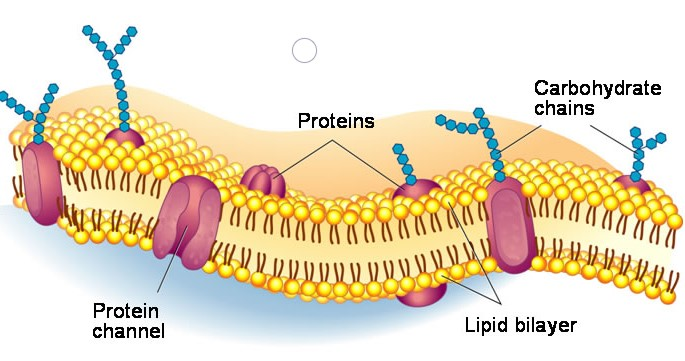
\includegraphics[width=\linewidth]{membrane.jpg}
				
			\end{figure}
		\end{minipage}
		\hspace{0.05\linewidth}
		\begin{minipage}{0.45\linewidth}
			\begin{figure}[H]
				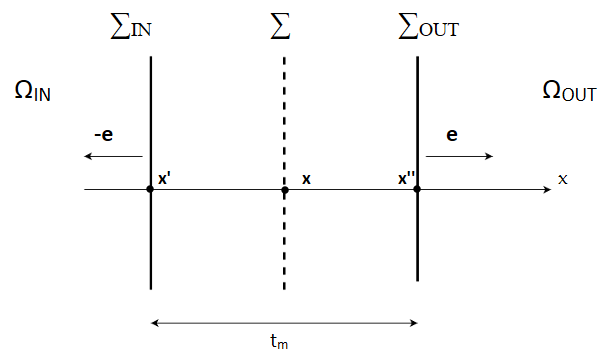
\includegraphics[width=\linewidth]{intra.png}
				
			\end{figure}
		\end{minipage}
		
	\end{minipage}
	\caption{\textit{Left: schematic representation of the cellular membrane.
			Right: mathematical description of the cellular membrane}}
\end{figure}



\begin{figure}[H]
	\begin{center}
		\begin{tabular}{ |c|c|c|c| } 
			\hline
			\textbf{Electric quantity} & \textbf{Name} & \textbf{Unit measure} \\
			\hline
			$t_m$ & Membrane thickness & $m$ \\ 
			\hline
			$R_c$ & Cell radius & $m$ \\
			\hline
			$\psi_m$ & Membrane potential & $V$ \\
			\hline
			$J$ & Current density & $A/m^2$ \\
			\hline
			$I$ & Current & $A$ \\
			\hline
			$\sigma$ & Surface charge density & $C/m^2$ \\
			\hline
			$c_m$ & Specific membrane capacitance & $F/m^2$ \\
			\hline
			$C_m$ & Membrane capacitance & $F$ \\
			\hline
			$g_m$ & Specific membrane conductance & $S/m^2$ \\
			\hline
			$G_m$ & Membrane conductance & $S$ \\
			
			\hline
		\end{tabular}
		
	\end{center}
	\caption{Main electrical quantities in cellular electrophysiology}
\end{figure}
	
	
\subsection{ODE local and global models}
	
	\begin{figure}[H]
		\begin{minipage}{\linewidth}
			\centering
			\begin{minipage}{0.45\linewidth}
				\begin{figure}[H]
					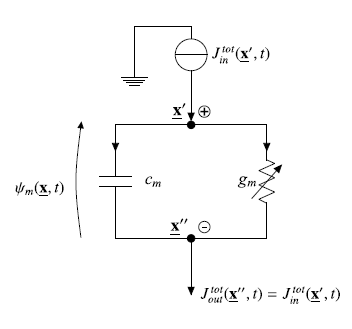
\includegraphics[width=\linewidth]{ode_circuit.png}
					
				\end{figure}
			\end{minipage}
			\hspace{0.05\linewidth}
			\begin{minipage}{0.48\linewidth}
				\begin{figure}[H]
					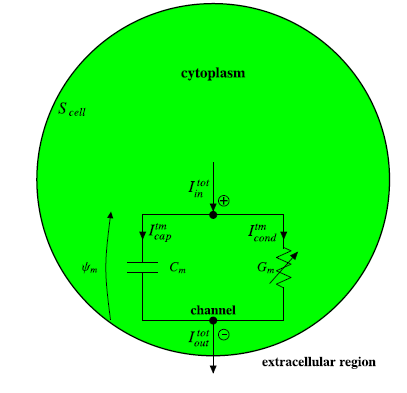
\includegraphics[width=\linewidth]{global_circuit.png}
					
				\end{figure}
			\end{minipage}
			
		\end{minipage}
		\caption{\textit{Left: equivalent circuit for a fixed point $\textbf{x} \in \Sigma$ (local model)  \\
				Right: equivalent circuit for the whole membrane  $\Sigma$ (global model)}}
	\end{figure}

	
	Considering  a point $\textbf{x} \in \Sigma$, equation (1) expresses a balance law for the current densities $J^{TOT}$, which can be divided in two contributions (capactive and conduction), where the capacitive current assumes the form $J^{cap}(\textbf{x},t) = c_m \frac{\partial \psi_m(\textbf{x},t)}{\partial t}$.\\
	The conduction current takes the general form 
	
	\begin{equation}
		J^{cond}_{\alpha}(\textbf{x},t) = g_m(\textbf{x},t,\psi_m(\textbf{x},t)) [\psi_m(\textbf{x},t) - E_{c,\alpha}]
	\end{equation}
	
	where $g_m$ is the \textbf{specific conductance}, depending on $\psi_m$, and $E_{c,\alpha}$ is the \textbf{Nernst potential}, which corresponds to the  membrane potential for which the ion conduction current is equal to $0$.\\
Such expressions for the current densities can be syntethized in a \textit{circuital form} of equation (1), in which their two contributions (capacitive and conduction) are modeled respectively through a specific capacitance and a specific conductance (see Figure). Then, an application of the Kirchhoff current law  gives the current balance for the circuit.\\
For any fixed $\textbf{x} \in \Sigma$,  equation (9) is an \textbf{ordinary differential equation (ODE)} in the unknown $\psi_m$. This model is a \textit{local} model, since the focus has been on a specific point of the membrane $\textbf{x}$.
\\
	If instead of a specific $\textbf{x} \in \Sigma$, the aim is to write a current balance across the whole cell's membrane $\Sigma$, the resulting differential equation, which in this case expresses a \textit{global} whole cell model, is obtained by integration of (9) over the surface $\Sigma$,  which yields the conservation of the total current 
	
	\begin{equation}
		I_{\alpha}^{TOT} = \int_{\Sigma} \textbf{J}_{\alpha}^{TOT} \cdot \textbf{n}_{out} dS 
	\end{equation} 
In this case, we need to define the whole cell membane conductance $ G_m$ and capacitance $ C_m $, so that the current balance takes the form

\begin{equation}
	I_{\alpha}^{TOT}(t) = I_{\alpha,in}^{TOT}(t) =I_{\alpha,out}^{TOT}(t) = I_{\alpha}^{cap}(t) + I_{\alpha}^{cond}(t)
\end{equation}
	
where $  I_{\alpha}^{cap}(t) = C_m \frac{d \psi_m(t)}{d t}$ and $ I_{\alpha}^{cond}(t) = G_m(t,\psi_m) [\psi_m(t) - E_{c,\alpha}]$.\\
While the (specific) capacitance is an intrinsic value of the cell, the conduction current, and  in particular the (specific) conductance $G_m$, need to be modeled. In the next sections, three main models used in literature for this purpose will be presented: the \textbf{linear resistor model (LRM)}, the \textbf{Goldman-Hodgkin-Katz (GHK)} model and finally the \textbf{Hodgkin-Huxley (HH)} model.\\


	
	
\subsection{The LRM model}

\begin{figure}[H]
	\begin{center}
		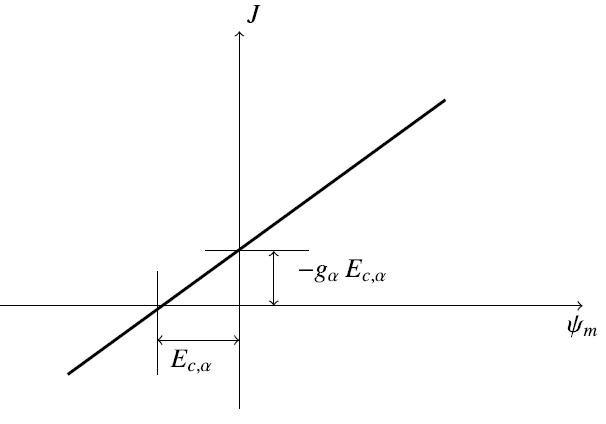
\includegraphics[scale=0.77]{LRM.png} 
	\end{center} 
	\caption{\textit{Characteristic curve for the linear resistor model}}
	
\end{figure}

The \textbf{linear resistor model (LRM)} makes the simplest assumptions 

\begin{equation}
	g_{m,\alpha}(\textbf{x},t,\psi_m(\textbf{x},t)) = g_{m,\alpha}^0 = const \hspace{1.5 cm} E_{c,\alpha}(\textbf{x},t) := E_{c,\alpha}^0 = const \hspace{1cm} \forall \alpha
\end{equation}

Therefore, this model assumes the conductance and the Nernst potential as constant.
The resulting expression for the conduction current is
\begin{equation}
	i_G(t) = g_{m,\alpha}^0 [\psi_m -  E_{c,\alpha}^0]
\end{equation}

This law defines a straight line in the plane $i_G$ vs $\psi_m$, such that there exists a unique value of membrane potential for which $i_G=0$. This value is exactly the Nernst potential $E_{c,\alpha}^0$ .


The Nernst potential $E_{c,\alpha}^0$is related to the concept of  \textbf{thermodynamic equilibrium}. Micorscopic theory assumes that ion particles in the channel are subjected to two different contributions: diffusion process caused by the chemical gradient, and a transport caused by the presence of an \textit{electrical field} $\textbf{E}(\textbf{x},t)$ [Sacco-Guidoboni]. This phenomenological perspective leads to the \textbf{drift-diffusion (DD)} model for the conduction current density, which reads

\begin{equation}
	\textbf{J}_{\alpha}^{DD} = \textbf{J}_{\alpha}^{DIFF} + \textbf{J}_{\alpha}^{DRIFT} = -Fz_{\alpha}D_{\alpha}\nabla C_{\alpha} + F|z_{\alpha}| C_{\alpha}\mu_{\alpha}\textbf{E}
\end{equation}
where 
\begin{itemize}
	
	\item $F$ is the \textbf{Faraday constant}, such that $F = q N_{av}$, being $q$ the elementary charge and $N_{av}$ the Avogadro's constant
	
	\item $z_{\alpha}$ is the \textbf{ion number}, positive for cations and negative for anions
	
	\item $\mu_{\alpha}$ is the \textbf{ion electrical mobility}
	
	\item $C_{\alpha}$ is the molar density of ion $\alpha$
	
	\item $D_{\alpha}$ is the \textbf{ion diffusivity}. this value can be retrieved from the \textit{Einstein-Smoluchowki} relation [Md. Akhtarul Islam] $D_{\alpha} = V_{TH}\frac{\mu_{\alpha}}{|z_{\alpha}|}$, where $ V_{TH} \sim 26 mV$ is the \textit{thermal voltage}
\end{itemize}

\begin{theorem}
	Let us assume one dimensional gemetry. Then, the thermodynamic equilibrium, for which $\textbf{J}_{\alpha}^{DD} = 0$ and  the drift current density balances the diffusion current density, is obtained at the value of potential

\begin{equation}
	E_{c,\alpha}^0 = \frac{V_{TH}}{z_{\alpha}}\ln\left(\frac{C_{\alpha}^{OUT}}{C_{\alpha}^{IN}}\right)
\end{equation}	


\end{theorem}




\subsection{The GHK model}
With the \textbf{Goldman-Hodgkin-Katz (GHK)} model, the modeling of the conduction current becomes nonlinear. Here, the following assumptions are adopted: 

\begin{itemize}
	
	\item The electric field in the ionic channels assumes a constant value of $ E = \frac{\psi_m}{t_m}$, i.e. the ratio between the membrane potential and the membrane thickness
	
	\item The geometrical setting is one dimensional
	
	\item The conduction current $\textbf{J}_{\alpha}^{cond}$ varies only in time, i.e. is constant in space and $ \frac{\partial J_{\alpha}^{cond} }{\partial x} = 0$. This means that there is no production or consumtpion of ions along the channel
	
\end{itemize}

Applying these hypothesis to eq.15, it can be shown that the conduction current density takes the form

\begin{equation}
	J_{\alpha}^{GHK}(\psi_m,t) = -qz_{\alpha}P_{\alpha}\left[n_{\alpha}^{out} \mathcal{B}(\beta_m) - n_{\alpha}^{in} \mathcal{B}(-\beta_m) \right]
\end{equation}

where $P_{\alpha} = \frac{D_{\alpha}}{t_m}$ is the \textbf{membrane permeability}, $ \beta_m := \frac{z_{\alpha} \psi_m}{V_th}$ and $ \mathcal{B}(x) = \frac{x}{e^x -1}$ is the \textbf{inverse Bernoulli function}.\\
It can be proven [Sacco-Guidoboni] that (17) can be written in general form (10) by setting:

\begin{equation}
	g_{\alpha}(\psi_m,t) = P_{\alpha}\frac{q z_{\alpha}^2N_{av}C_{\alpha}^{in}(t)}{V_{TH}} 
\end{equation}

\begin{equation}
E_{eq}(\psi_m,t) = P_{\alpha}\frac{V_{TH}}{z_{\alpha}} \left(\frac{C_{\alpha}^{out}(t)}{C_{\alpha}^{in}(t)} - 1\right)\mathcal{B}(\beta_m)
	\end{equation}
	
	
	
	\subsection{The Hodgkin-Huxley model}
	
	\begin{figure}[H]
		\begin{center}
			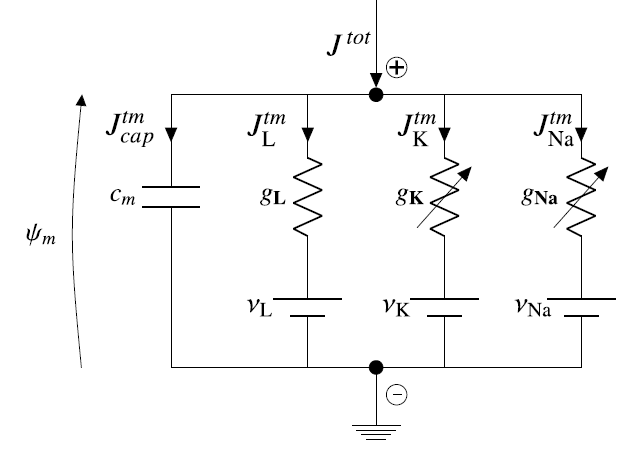
\includegraphics[scale=0.9]{HH.png} 
		\end{center} 
		\caption{\textit{Equivalent circuit for the Hodgkin-Huxley model}}
		
	\end{figure}


In 1963, Hodgkin and Huxley (HH) published in a paper a revolutionary work, which awarded them the Nobel prize, on mathematical modeling of the electrophyisiogical activity of cells, with the focus on the neurons of the giant squid [Hodgkin-Huxley]. The equivalent circuit of the HH model is shown in Figure. The main assumptions of the model can be resumed as follows:

\begin{itemize}
	
	\item The total current density $J^{tot}$ can be split in two contributions: a capacitive transmembrane current $J_{cap}^{tm} = c_m \frac{\partial \psi_m}{\partial t}$, where the capacitance is assumed to be a constant quantity, and, for every ion considered, a conduction transmembrane current  $J_{cond}^{tm}$ to be modeled. The main ions considered are \textit{potassium} ($K^+$) and \textit{sodium} ($Na^+$). The remaining contribution is mostly due to \textit{chlorine} ($Cl^-$) and is summarized in a \textit{leakage} current $J_L^{tm}$
	
	\item With every ion $\alpha$ is associated its Nernst potential $E_{c,\alpha}$, representing the value for which thermodynamic equilibrium is achieved for each ion current density
	
	\item In order to better describe what happens at a biological level of the cell membrane, the ionic channel have a \textit{state}, i.e. an associated probability value which tells the percentage of their opening. Indeed, the behaviour of ionic exchange between the cytoplasm and the extracellular environment, strongly depends on the closing and opening of the ionic channel. With the HH model, the attempt is to mathematrically describe the opening status of the channel along time
	
	
\end{itemize}	


In the original form of the paper, a change of variable is performed: let us define the equilibrium potential of the whole cell as $E_m$, and define for every ion $\alpha$ the quantities

\begin{equation}
	v_\alpha := E_{c,\alpha} - E_m \hspace{2cm}  v := \psi_m - E_m
\end{equation}
	
	In this way, the form of the current density of ion $\alpha$ becomes
	
	
	\begin{equation}
	J_\alpha^{cond} = g_{m,\alpha}(v-v_\alpha)
	\end{equation}
	
	and the Kirchhoff current law for the circuit, expressed for the new variable $v = v(t)$, is
	
	\begin{equation}	
	\begin{cases}
	J^{tot} = c_m \frac{\partial v}{\partial t} + g_{Na}(v - v_{Na}) + g_{K}(v - v_{K}) +g_{L}(v - v_{L})  \\
	v(0) = 0
	\end{cases}	\end{equation}
	
	
	having assumed the membrane potential at equilibrium at time $t=0$.\\
	For the whole equilibrium potential $E_m$, the \textbf{Goldman potential} can be used [Ermantraut-Terman]
	
	
	\begin{equation}
	E_m= V_{TH} \ln \left[\frac{P_{Na} C_{Na}^{out} + P_{K} C_K^{out} + P_{Cl} C_{Cl}^{in}}{P_{Na} C_{Na}^{in} + P_{K} C_K^{in} + P_{Cl} C_{Cl}^{out}}\right]
	\end{equation}
	
	where $P_\alpha$ and $C_\alpha$  denote the permeability and molar density of ion $\alpha$, respectively.\\
	As for the modeling of conductances, let us introduce the \textbf{gating variables} $n,m,h$ for the three considered ion species $K^+,Na^-,Cl^-$. They represent the probability of opening of the ionic channel. For example, if the cell is in a situation in which $C_{Na}^{out} > C_{Na}^{in}$, the opening of $Na^+$ channel will result in a current flow from outside to inside, and to a corresponding rise of the potential $\psi_m$. When the membrane potential reaches the value of equilibrium $E_{Na}$, the sodium channel will close. For this reason, the gating variables are expressed as the solution of ordinary differential equation of the type
	
		\begin{equation}
	\frac{dy}{dt} = \gamma (1-y) - \delta y \hspace{1 cm} \gamma,\delta >0  \hspace{1 cm} y = m,n,h
	\end{equation}
	
	so that there is a balance between a production rate $\gamma$ and a consumption $\delta$. The solution of an ODE in this form is
	
	\begin{equation}
	y(t) = y_\infty \left[1 - \exp\left(\frac{-t}{\tau}\right)\right]
	\end{equation}
	
	where
	
	\begin{equation}
	y_\infty = \frac{\gamma}{\gamma + \delta} \hspace{1.5cm} \tau = \frac{1}{\gamma + \delta}
	\end{equation}
	
	For the potassium conductance, the chosen dependence on its gating variable (in agreement with experimental data) is $ g_K = \bar{g}_K n^4$. For the sodium variable, it has been observed that also a second process was involved, so that the proposed form is  $ g_{Na} = \bar{g}_{Na} m^3h$. The values $\bar{g}_K$ and $\bar{g}_{Na}$ are constant and determined to fitting of experimental data.\\
	To summarize, the HH model consists in the following sytem of nonlinear ordinary differential equations:
	
	\begin{equation}
		\begin{cases}
		J^{tot} = c_m \frac{d v}{d t} + J_{Na} + J_K +J_L  & \text{(Kirchoff current law)}\\
		J_\alpha = g_\alpha (v-v_\alpha) \hspace{1 cm}  \alpha = Na,K,Cl & \text{(Conduction current densities)}\\
		\frac{dn}{dt} = \gamma_n(1-n) - \delta_n n & \text{(ODE for gating variable n)} \\
		\frac{dm}{dt} = \gamma_m(1-m) - \delta_m m & \text{(ODE for gating variable m)}\\
		\frac{dh}{dt} = \gamma_h(1-h) - \delta_h h & \text{(ODE for gating variable h)}\\
		 g_K = \bar{g}_K n^4 & \text{(Modeling conductance for K)}\\
		 g_{Na} = \bar{g}_{Na} m^3h  & \text{(Modeling conductance for Na)}
		
		\end{cases}
	\end{equation}
	
	\begin{figure}[H]
		\begin{center}
			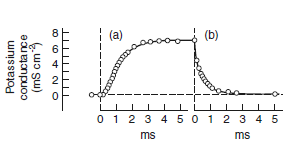
\includegraphics[scale=1.1]{gk.png} 
		\end{center} 
		\caption{\textit{Example of behaviour of the potassium conductance $g_K$: a step increase is followed by a decrease. The dots are experimental data}}
		
	\end{figure}


\subsection{Cable model}

\begin{figure}[H]
	\begin{center}
		\hspace*{-0.7cm}
		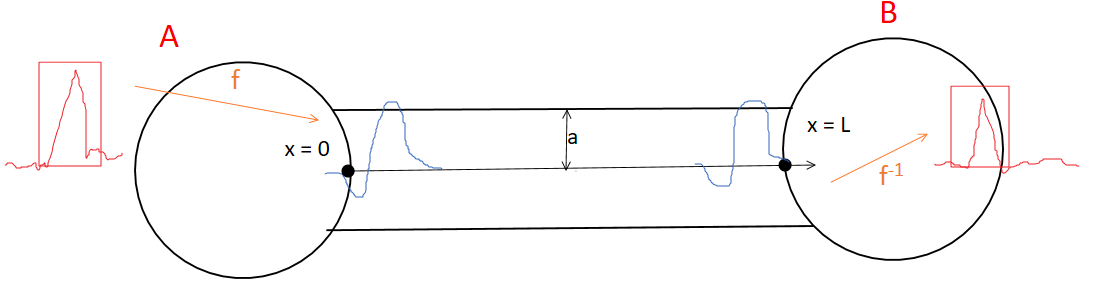
\includegraphics[scale=0.7]{cable.png} 
	\end{center} 
	\caption{\textit{Schematic representation of the cable model}}
	
\end{figure}


The models studied so far described the dynamic evolution of the membrane potential  for a single cell. In order to go further, we need to keep into account also the \textit{communication} between two cells, i.e. the propagation of the action potential from one neuron to another. Biologically, this propagation is mediated by the \textit{axon} connecting the two units. The axon is sa part of the neuron, and at its every point we may assume a communication with the surrounding environment through electrical circuits as described in the previous sections.\\
The main assumptions for the cable model are the following:

\begin{itemize}
	
	\item The biological cable, i.e. the axon, has length $L$ and radius $a$ (thus a cross-sectional area  $S=\pi a^2$), with $\frac{a}{L} << 1$, allowing us to represent the cable as a $1D$ object along a longitudinal axis $ x \in [0,L]$
	
	\item The electric potential outside the cell is constant, as well as the concentrations inside and outside the cell for every ion $\alpha$: 
	$$ \psi^{out}(x,t) = const  \hspace{1cm} C_\alpha^{in}(x,t)  = const \hspace{1cm} C_\alpha^{out}(x,t)  = const$$
	
	\item The \textbf{resistivity} of the axon $\rho_{ax}$ is constant. The resitivity is the reciprocal of the \textit{conductivity} $\sigma$, and is related to the \textit{resistance} $R_{ax}$ by $ R_{ax} = \frac{\rho_{ax} L}{S}$
	
	
\end{itemize}


If we consider an element of length $dx$ of the cable, its contribution to resistance is $dR(x) = \frac{\rho_{ax} dx}{\pi a^2}$. If a current $I_{in}$ enters the element, the consequent potential difference across the element is $ d\psi_m(x,t) = - \left(\psi_m(x+dx,t) - \psi_m(x,t)\right) = dR(x)I_{in}(x,t) = \frac{\rho_{ax} dx}{\pi a^2} I_{in}(x,t)$. Therefore, letting $dx \rightarrow 0$, this implies that

\begin{equation}
	I_{in}(x,t) = -\frac{\pi a^2}{\rho_{ax}}\frac{\partial \psi_m(x,t)}{\partial x}
\end{equation}

Next, to express a current balance at each point $x$, we need to consider again an infinitesimal element $dx$, in which a current $I_{in}(x,t)$ is entering the element, a current $I_{in}(x+dx,t)$ is leaving the element, and a transmembrane current $I_{TM}(x+\frac{dx}{2},t)$ is flowing from the axon to the extracellular environment, with a capacitive and a conduction contributions [see Figure].\\
The application of Kirchhoff current law at the node  $x+\frac{dx}{2}$ gives

\begin{equation}
- I_{in}(x,t) + I_{cap}(x+\frac{dx}{2},t) + I_{cond}(x+\frac{dx}{2},t) + I_{in}(x+dx,t) = 0
\end{equation}

The capactive and conductive contributions to the transmembrane current are
\begin{equation}
  I_{cap}(x+\frac{dx}{2},t) = J_{cap}(x+\frac{dx}{2},t) 2 \pi a dx = c_m \frac{\partial \psi_m(x,t)}{\partial t} 2 \pi a dx 
\end{equation}

\begin{equation}
I_{cond}(x+\frac{dx}{2},t) = J_{cond}(x+\frac{dx}{2},t) 2 \pi a dx 
\end{equation}

where $J_{cond}$ can be mathematically described using any of the LR, GHK or HH models. Dividing equation (28)  by $2 \pi a dx $ and letting $dx \rightarrow 0$ gives rise to the equation system

\begin{equation}
\begin{cases}
\frac{\partial \psi_m(x,t)}{\partial t} + \frac{1}{2 \pi a }\frac{\partial I_{in}(x,t)}{\partial x} + J_{cond}(x,t) = 0 \\
I_{in}(x,t) = -\frac{\pi a^2}{\rho_{ax}}\frac{\partial \psi_m(x,t)}{\partial x}
\end{cases}
\end{equation}

The balance law (32) is a \textit{parabolic partial differential equation} for the unknown membrane potential $\psi_m(x,t) $, varying along space and time. To be solvable, (32) needs to to be completed with an initial condition $ \psi_m (x,0) = \psi_m^0(x)$ and appropriate boundary conditions. The nature of the cable equation will be linear or nonlinear depending on the chosen model for $J_{cond}$.\\
As for the boundary conditions, a common choice is to consider \textit{Robin boundary conditions}. Defining the potential at $x=0$ as $\bar{V}_{in}(t)$ and modeling the right-hand terminal of the axon through a resistance $R_{out}$, the resulting boundary conditions are

\begin{equation}
\begin{cases}
\psi_m(0,t) = \bar{V}_{in}(t) \\
-I_{in}(L,t) +\frac{1}{R_{out}}\psi_m(L,t) =0
\end{cases}
\end{equation}

\begin{figure}[H]
	\begin{center}
		
		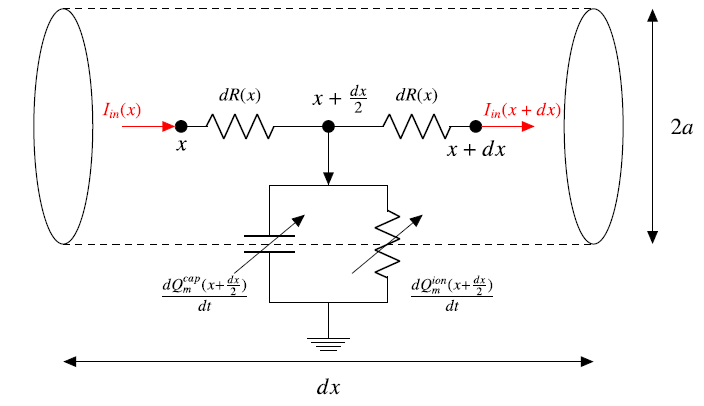
\includegraphics[scale=0.5]{curr_bal.png} 
	\end{center} 
	\caption{\textit{Current balance in an element $dx$ of the axon}}
	
\end{figure}

\subsection{Numerical solution of the cable equation}


\begin{figure}[H]
	\begin{center}
		
		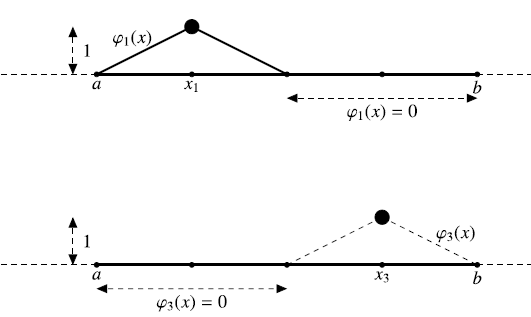
\includegraphics[scale=0.7]{basis.png} 
	\end{center} 
	\caption{\textit{Lagrangian basis functions}}
	
\end{figure}


The cable equation model is an example of the following one-dimensional \textit{diffusion-reaction} boundary value problem for unknowns $ u(x,t)$ and $\textbf{J} = J(x,t)\textbf{e}$:


\begin{equation}
\begin{cases}
\frac{\partial u}{\partial t} +\frac{\partial J}{\partial x} = \mathcal{P} & \forall (x,t) \in (0,L) \times (0,T) \hspace{1cm} \text{(Conservation law)} \\
J = - \mu \frac{\partial u}{\partial x} & \forall (x,t) \in (0,L) \times (0,T) \hspace{1cm} \text{(Flux law)}\\
u(x,0) = u^0(x) & \forall x \in (0,L) \hspace{1cm}  \text{(Initial condition)} \\
\gamma \textbf{J} \cdot \textbf{n} = \alpha u - \beta &  \forall (x,t) \in \partial \Omega \times (0,T) \hspace{1cm} \text{(Boundary conditions)}
\end{cases}
\end{equation}

Here, $\textbf{J}$  represents a \textit{flux} taking into account the diffusion, while $\mathcal{P}$ takes into account the  net production rate. The boundary coefficients $\alpha, \beta, \gamma$, depending on their values, can give rise to the main types of boundary conditions (Dirichlet, Neumann, Robin).\\
In order to numerically solve equation (33), the following two main steps need to be performed:

\begin{enumerate}
	\item \textbf{Time semidiscretization}. The time derivative is approximated with a finite-difference scheme. In the present case, the \textbf{Backward Euler method (BE)} is chosen, because of its unconditional stability [Quarteroni-Sacco]. Dividing the interval $[0,T]$ in $N_T$ subintervals of the form $[t^k, t^{k+1}]$ with $ k=0, \dots N_T-1$, and setting $\Delta t = \frac{T}{N_T} $, the semidiscretization of (33) using BE reads
	
	\begin{equation}
	\begin{cases}
	\frac{u^{k+1} - u^k}{\Delta t} +\frac{\partial J^{k+1}}{\partial x} = \mathcal{P}^{k+1}  \\
	J^{k+1} =  - \mu \frac{\partial u^{k+1}}{\partial x} 
	\end{cases}
	\end{equation}
	 
	where, for a scalar quantity $\phi(x,t)$, it has been used the notation $ \phi^k := \phi(x,t^k) $. The first equation of (34) can be rewritten as
	
	\begin{equation}
	\sigma ^{k+1} u^{k+1} +\frac{\partial J^{k+1}}{\partial x} = f^{k+1} 
	\end{equation}
	
	\item \textbf{Spatial discretization}. A Galerkin-FEM strategy is adopted to solve (34).Assuming, without loss of generality, $\gamma = \beta = 0$ and $\alpha =1$, and setting $V = H_0^1(0,L)$,  problem (34) can be rewritten in its \textit{variational form} [Quarteroni]
	
	\begin{equation}
	\text{Find $u \in V$ s.t.} \hspace{0.5cm} B(u,\varphi) = F(\varphi) \hspace{0.5cm} \forall \varphi \in V
	\end{equation}
	
	in which we have defined the forms
	\begin{equation}
	B(u,\varphi) = \int_{\Omega}\left[\mu \frac{\partial u}{\partial x}  \frac{\partial \varphi}{\partial x} + \sigma u \varphi \right]  dx
	\end{equation}
	
	\begin{equation}
F(\varphi) = \int_{\Omega} \left[f \varphi\right] dx
	\end{equation}
 Lax-Milgram theorem [Quarteroni] ensures existence, uniqueness and stability for the solution of (36).\\
 With the \textbf{Finite element method (FEM)}, the infinite dimensional setting of (36) is approximated by the introduction of a finite dimensional space $V_h$ s.t . $dim(V_h) = N_h < \infty$. For the present case, the chosen space is the linear combination of piecewise linear polinomials. Partitioning the interval $[0,L]$ into $M_h$ subintervals of uniform length $ h = \frac{L}{M_h}$ and indicating with $\tau_h$ the collection of subintervals, we define the space
 $$ V_h := \left\{ w_h\in C^0(\Omega) \hspace{0.5 cm} s.t. \hspace{0.5 cm} w_h|_{K_i} \in \mathbb{P}^1(K_i) \hspace{0.3 cm} \forall K_i \in \tau_h, \hspace{0.3 cm} w_h(0)=w_h(L)=0 \right\}$$
 
 where $ \mathbb{P}^1(K_i)$ is the set of linear polinomials defined on the interval $K_i$. The space $V_h$ is therefore a finite dimensional approximation of the space $H_0^1(0,L)$. Using for $V_h$ the \textit{Lagrangian basis} $ \left\{ \varphi _j \right\}_{j=1}^{N_h}$, where $ \varphi_j(x_i) = \delta_{ij}$, every element $w_h \in V_h$ can be written as
 
\begin{equation}
 w_h = \sum_{j=1}^{N_h} w_j \varphi_j(x)
\end{equation}

In light of this, the FE discrete formulation becomes

	\begin{equation}
\text{Find $u_h = \sum_{j=1}^{N_h} u_j \varphi_j(x) \in V_h$ s.t.} \hspace{0.5cm} B(u_h,\varphi_i) = F(\varphi_i) \hspace{0.5cm} \forall i = 1, \dots N_h
\end{equation}
resulting in the \textit{algebraic system}

\begin{equation}
B \textbf{u} = \textbf{F}
\end{equation}
where $\textbf{u} = [u_j]_{j=1}^{N_h}$, $B_{ij} = B(\varphi_j,\varphi_i)$ and $F_i = F(\varphi_i)$. The following theorem expresses the convergence of the FEM solution to the exact solution of (ref 36) [Quarteroni]:
\begin{theorem}[Convergence]
	Let $u \in H^2(\Omega) \cap H_0^1(\Omega)$. Then there exist two constants $c_1,c_2 >0$, independent of $h$, such that
	$$||u-u_h||_{H_0^1} \le c_1h||u||_{H^2}$$
	
	$$||u-u_h||_{L^2} \le c_2h^2||u||_{H^2}$$
\end{theorem}
\end{enumerate}

The above error estimates express the property that $u_h$ converges to $u$ with order $1$, with respect to $h$, in the $H^1$ norm, and with order $2$ in the $L^2$ norm, respectively.\\
The application of this discretization procedure to the cable equation (ref eq.) will results in a different algebraic system (41) depending on the adopted modeling of  $J^{cond}$. If a linear resistor model is adopted, the PDE, and consequently the algebraic system, will be linear. On the opposite side, if a nonlinear model is adopted, the nonlinearity will reflect also on the algebraic formulation. To this purpose, functional iterations can be adopted to iteratively solve the obtained nonlinear system, such as in the \textit{Newton method} or the \textit{Alternative lagging method} described in [Sacco-Guidoboni].

\end{document}
